\section{Analysis of Motor Data}
\label{sec:analysis}

\subsection{Motor components and setup}

\begin{figure}
    \centering
    \begin{circuitikz} 
    \draw (0.9,0.75) node[left] {5 V};
    \draw (5.5,0) node[left] {2};
    \draw (5.5,1) node[left] {1};
    \draw (5.5,-1) node[left] {3};
    \draw (10.5,0) node[left] {V$_2$ out};
    \draw (10.5,1) node[left] {V$_1$ out};
    \draw (10.5,-1) node[left] {V$_3$ out};
    \draw
    (0,0) to[battery]  (1,0)
          to[generic]  (9,0) -- (9,0)
          to[short,-o] (9,0)
    ;
    \draw
    (2,0) to[ground] (2,1)
          to[generic] (8,1) -- (8,1)
              to[short,-o] (9,1)
    ;
    \draw
    (2,0) to[ground] (2,-1)
          to[generic] (8,-1) -- (8,-1)
          to[short,-o] (9,-1)
    ;
    \draw
    (8,1) to[short] node[ground] {} (8,-3)
    ;
    \end{circuitikz}
    \caption{Caption}
    \label{fig:my_label}
\end{figure}

A basic DC motor consists of a stator, a rotor, a commutator, an external magnetic field, brushes, bearings and a shaft. A DC power supply is connected across the brushes, transmitting power through the commutator into windings around the rotor. The current flowing through the windings interacts with the permanent magnetic field producing a Lorentz force resulting in a torque across the windings. LORENTZ FORCE HERE

As the rotor spins away from a position with the windings perpendicular to the magnetic field, the torque is reduced. To allow a rotational force over the full revolution, commutators invert the current flow periodically. 

In the simplest possible motor, the rotor is composed of only one set of windings, with a split ring commutator inverting the power supply every half rotation. A more efficient model is to have multiple windings that receive power throughout different stages in the rotation. (figure here comparing 2 pole to multipole) This allows maximum torque to be applied throughout the entire rotation.

The brushes of a motor can be either spring loaded carbon rods, or copper strips pressed against the commutator. Carbon rods are far more efficient and less damaging to the motor, the reasons for this will be discussed further. With advancements in technology, brushless DC motors are becoming increasingly popular, removing the inefficiencies induced by the traditional brushes. 

Mechanical components, such as the bearings, shaft or motor housing are prone to physical damage. This could be due to either physical trauma or a contamination within the motor during operation. Failure of this type would need heavy repairs, with sometimes expensive replacements necessary, it is therefore important to diagnose any unhealthy running motor to minimise the damage.

The vibrational data collected by the contact microphones provided an analogue output, which when passed through a NI QAQ box, could be converted and saved as a csv file. The circuit diagram showing the configuration of components is displayed in….figure here

%Each motor component, what it does and how they fail.

%How the data collected by the sensors is connected to the DAQ box so that it can be used.

\subsection{Baseline Test}

\subsection{Overheating}

Overheating is widely regarded as the most common cause of motor failures, with many other types of motor deterioration leading to overheating. This is such a substantial problem that a rise of just 10 $^o$C above the regular running temperature causes the life expectancy of the motor to halve. The life span is halved once again for every 10 $^o$C the temperature is raised further.

The problem arises as, during overheating, the varnish covering the metal wires begins to melt. If this occurs at two points of wires that are in contact, the coil of the motor can short circuit.

%(Gears Removed motor)

In order to induce motor failure, a motor, shown in Figure.~\ref{fig:hotplate_motor}, consisting of 7 coils separately providing power was placed on a hotplate, heated to 150 $^o$C, for one hour. This was compared to the assumed usual running temperature of 60 $^o$C, meaning that just one hour on the hot plate equated to 512 hours of regular use.

For this failure mode, only coil was in direct contact with the plate so as only to damage that coil, leaving the others, ideally, with little impairment. Despite the fact that some heat would obviously be conducted through the motor, the effect of this was considered to be minimal with respect to the effect on the targeted coil.

The result of just one coil being broken is that there would be a brief loss of power in the motor when this coil was in contact with the brushes. %Brushes????
Therefore the speed of revolution would no longer be uniform. This can cause other problems to occur in the motor such as damage to the bearings.

\begin{figure}[t]
    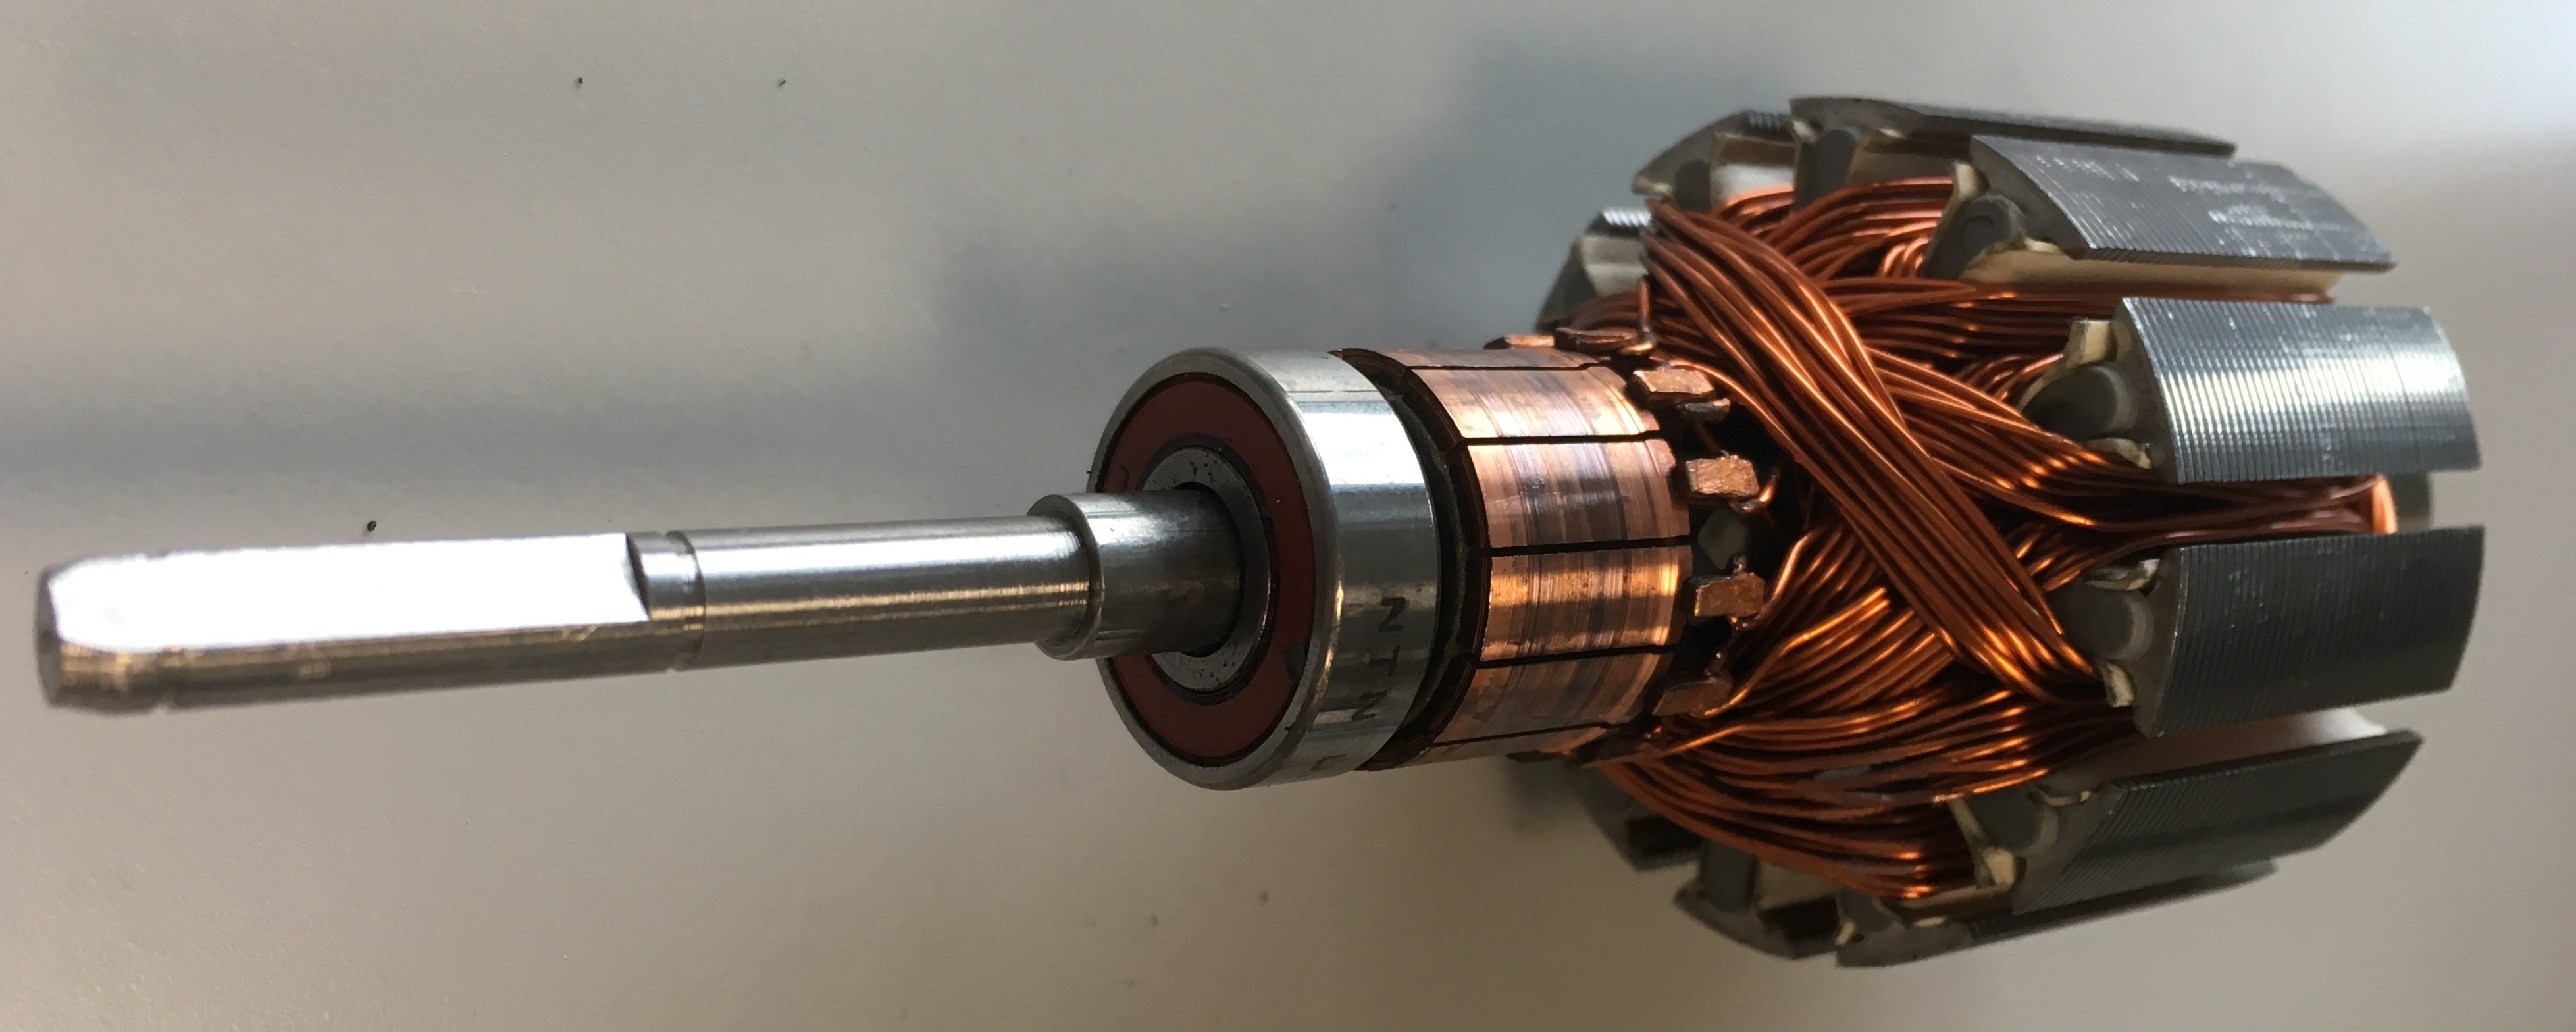
\includegraphics[width=1.0\textwidth]{fig/Gears_Removed_Inside.png}
    \caption[Time Domain]{The inside of the Gears removed motor showing the 7 separate coils, one of which was placed directly on the hotplate at 150$^o$C for one hour to induce failure.}
    \label{fig:hotplate_motor}
\end{figure}

In addition to this, the motor was placed in an oven at 200 $^o$C for 2 hours to cause extensive damage to all the coils evenly. This equates to over 30,000 hours of running in regular conditions. This was considered sufficient to bring the motor very close to failure given the typical life span of a motor is just 1000 hours. %1000???
Data was then collected for one minute to find any lasting damage.

%Need references from papers for this


\subsection{Overvoltage}

An increase in voltage will also cause an increase in current, resulting in more eddy currents in the wires and subsequently heating the motor. As stated earlier, this is a major reason for motor failures. 

Moreover, overvoltaging causes the torque of the motor to increase. The subsequent increased rotation speed leads to the motor %Which Part??? 
slipping. In order to reduce this slip, the motor will then draw an even greater current further contributing to the overheating effect. As well as this, a greater rotation speed will increase friction and will wear down bearings and brushes. Just a small increase in voltage can result in a large amount of damage as,

\begin{equation}
\tau \propto V^2,
\label{Torque}
\end{equation}

where $\tau$ is torque and $V$ is voltage.

In addition to the detrimental effect of overvoltaging, undervoltaging can be just as destructive. In fact, the effect of slipping is even more prominent when a motor is not given enough power and leads to more overheating.

%12V motor

The effect of overvoltaging  was investigated by running a 12 V motor at increasingly high voltages ranging from 12 V to 30 V. This was done for just one minute each time and was used to find the immediate effects of overvoltaging a motor.
    
%Large Motor

A second motor, also with a regular operating voltage of 12 V, was run at 30 V for one hour. In this instance, the bearings reached 90 $^o$C; this demonstrates the extreme effects of overvoltaging a motor. Readings could not be taken during this run as the sensors are only able to operate %Need synonym
up to 60 $^o$C. %Correct???
Therefore, readings were taken before and after the one hour run. This allowed us to explore the long term effects of overvoltaging a motor.

%Undervoltage experiment

%Do we need photos of these motors???

%Again need references.

\subsection{Load}

%Leads to overheating. Draws more current and voltage.

%Gripped shaft
    %This should produce an anomaly and show us what we are looking for.

%Fans in water, 1cm, 2cm, 3cm
    %12V Geared motor ran fine and didn't seem to struggle with the load even with the thickest fan.
    %Large motor was not geared and struggled to reach any voltage over 4V with 1cm fan.
        %Ran at 1-4V in water with 1cm fan.
    
\subsection{Misalignment}
%Motor shaft misaligned from the initial location, causing a non constant shaft rotation. Misalignment can cause damage to the bearings, the stator or the rotor due to knocking as it rotates, all leading to a final failure of the motor. Even small deviations from a perfectly aligned motor can cause damage, so detecting misalignment before damage occurs is important. 
\subsection{Brush Damage}
The brushes of a DC motor are a vital component, key to the proper working of the motor, allowing a DC power supply to provide an almost constant driving force throughout the entire revolution of the motor. The stationary brushes, combined with the rotating commutator attached to the rotor, periodically inverts the power supply throughout the revolutions. The commutator is composed of strips of conducting metal, usually copper, placed around the rotor. The strips of copper supply the current from the spring loaded brushes to the windings.  Without this periodic inversion of current direction through the windings, the motor would fail to spin and, as such, a good contact between the face of the brush and the commutator is necessary. 

The main cause of damage to the brushes of a DC motor usually occurs during maintenance. The soft surfaces of the carbon brushes can be easily scratched if not handled correctly. It is also possible that dirt can enter the motor housing during operation, which if found between the brush and the commutator, can cause heavy damage. In order to induce this type of failure mode, the brushes were treated with a heavy grit sandpaper, leaving the surface very rough. (picture of rough brushes here). 

It is possible for any imperfections in the surface of the carbon brushes to be removed without intervention during normal operation. As the rotor spins making contact with the face of the brushes, the friction generated is often capable of reducing the magnitude of the scratches. The possibility of this self repair will be investigated. However this friction of the brushes can cause another failure mode, loss of contact due to reduction in size of the brushes over time. This requires the brushes to be entirely replaced, making brushed motors unsuitable for use in remote locations. %more about self repair, what we did, e.g. left running for x volts for y time, more photos

The rough contact between the brush and commutator when damaged can cause sparking, leading to damaged commutators. Replacing the brush on a motor is a relatively simple maintenance task, however replacing the copper strips can be more complicated. It is therefore important to ensure that a motor running with damaged brushes is identified immediately, to prevent running in sub-optimal conditions, potentially causing further damage. (picture here of commutator on small 12V motor, this motor has copper strips for brushes, not carbon, so famously “sparky”)

Due to the flaws in the brushed DC motor model, their use has been declining with the introduction of brushless DC motors. These use an integrated switching power supply, to convert the DC to AC for the motor to run. Another alternative is to simply use an AC motor. 

%carbon rods
    %Contact surface with rods should be smooth for a healthy motor running in optimal conditions. Due to various causes, including damage during maintenance, these surfaces can become imperfect. Scratches on the surface of the brushes can result in an unhealthy running of the motor. The soft carbon in the rods can be worn down due to friction with the split ring as the motor rotates, this can lead to a self repair of the brushes with the scratches removed. This erosion of the brushes is a slow process, driven by friction, which will eventually lead to the brushes needing replacement. The friction created in the wear of the brushes generates heat which, when coupled with another failure mode such as overvoltage, can accelerate the degradation of the motor.
    %images of healthy/damaged brush
%Split ring:
    %Damage to the split ring that connects the brushes can occur, causing a faulty connection between the power supply and the coils. This causes an uneven rotation speed, with the power supplied being discontinuous. As above, this discontinuity interrupts the smooth running of a motor, with knocking becoming a factor. 
    %images of hammer on brushes vs normal brushes
\subsection{Gear Damage}

%First degreased the gears with a citrus degreasing spray.
%Added dirt to cause gears to break and prevent easy movement.
    %This can lead to overheating
%Placed in water for a few days to cause the motor to rust

\subsection{Specific Failures}

%Tapping sensors

%2 motors run in parallel with motors placed next to each other so that they vibrate against each other

Unlevel footing.

A motor running with soft footing can be the cause of multiple failures within a motor. When a motor with a misaligned shaft is coupled with an uneven motor housing, the uneven weight distribution as the rotor spins is exaggerated. The negative impacts of the uneven shaft are amplified, meaning even misalignments can now be damaging. 

The cause of a soft footing can be either an imperfection in the mounting feet of the motor, or the foundations the motor is mounted upon. In either case the motor will have the ability to move in a diagonal plane, similar to a chair or table on uneven ground, causing the shaft to become misaligned. This can be avoided by properly aligning the mountings and the foundations, commonly performed in industry using laser precision tools. 

This failure mode was induced by suspending the large motor above the work surface with a loosely gripped clamp stand. Any movement within the motor could cause a much larger movement in the stand, allowing the motor to oscillate while being suspended in the air. This oscillation will have an impact upon the shaft within the motor, exaggerating movements within the stator. The effects of this are similar to misalignment discussed above. Depending on the frequency of rotation of the motor, a resonance can occur, massively amplifying the oscillations causing an increased level of damage. If the feet do become loose, it is important to be aware of this before long term running of the motor is performed, as this would cause damage to internal components. It is more cost and energy effective to ensure proper footings prior to running.

    %When taking one reading, the vibrations of the motor were so great that it caused the whole clamp stand to move.